%%%%%%%%%%%%%%%%%%%%%%%%%%%%%%%%%%%%%%%%%
%
% (c) 2022 by Jennifer Laaser
%
% This work is licensed under the Creative Commons Attribution-NonCommercial-ShareAlike 4.0 International License. To view a copy of this license, visit http://creativecommons.org/licenses/by-nc-sa/4.0/ or send a letter to Creative Commons, PO Box 1866, Mountain View, CA 94042, USA.
%
% The current source for these materials is accessible on Github: https://github.com/jlaaser/pogil-polymers
%
%%%%%%%%%%%%%%%%%%%%%%%%%%%%%%%%%%%%%%%%%

\renewcommand{\figpath}{content/intro/measuring-MW/figs}
\renewcommand{\labelbase}{measuring-MW}

\begin{activity}{Measuring Molecular Weight}
\label{\labelbase}

\begin{instructornotes}

	This activity introduces students to key concepts related to methods used to measure the molecular weights and molecular weight distributions of polymers.
	
	After completing this activity, students will be able to:
			\begin{enumerate}
				\item Use end-group analysis via NMR and UV-Vis to calculate the number-average molecular weight of a polymer
				\item Qualitatively interpret the relative molecular weights and dispersities of polymers measured by SEC
				\item Interpret MALDI spectra in terms of the repeat unit mass and frequency of chain lengths, and calculate molecular weights and dispersities of polymer samples from MALDI data
			\end{enumerate}
			
	\subsection*{Activity summary:}
	\begin{itemize}
		\item \textbf{Activity type:} Learning Cycle
		\item \textbf{Content goals:} Measuring molecular weights
		\item \textbf{Process goals:} %https://pogil.org/uploads/attachments/cj54b5yts006cklx4hh758htf-process-skills-official-pogil-list-2015-original.pdf
			\begin{itemize}
				\item Interpreting graphs and numeric data
				\item Written and oral communication of reasoning
			\end{itemize}
		\item \textbf{Duration:} TBD
		\item \textbf{Instructor preparation required:} none beyond knowledge of relevant content
		\item \textbf{Related textbook chapters:}
			\begin{itemize}
				\item \emph{Polymer Chemistry} (Hiemenz \& Lodge): section 1.8
			\end{itemize}
		%\item \textbf{Facilitation notes:}
		%	\begin{itemize}
		%		\item \dots
		%	\end{itemize}
	\end{itemize}
	
\end{instructornotes}




\begin{model}[End Group Analysis]
\label{\labelbase:mdl:endgrpanalysis}

	One simple method for determining the molecular weight of a polymer is by \emph{end-group analysis}.
	
	To employ end-group analysis, the end-group(s) on each polymer chain must have a chemical or physical feature that can be detected and quantified independently of the rest of the polymer chain, as depicted below:
	
	\centerline{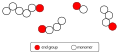
\includegraphics[width=0.5\textwidth]{\figpath/Model1-endgrp-schematic}}

\end{model}


\begin{ctqs}

	\question How many end groups are shown in the polymer sample depicted in Model \ref{\labelbase:mdl:endgrpanalysis}?
	
		\begin{solution}[0.25in]
			4
		\end{solution}
	
	\question How many monomers are shown in the polymer sample depicted in Model \ref{\labelbase:mdl:endgrpanalysis}?
	
		\emph{Note: for the purposes of this question, do not count the end group beads as monomers.}
	
		\begin{solution}[0.25in]
			12
		\end{solution}
	
	\question Calculate the average degree of polymerization of the polymer sample depicted in Model \ref{\labelbase:mdl:endgrpanalysis} by dividing your answer to part (b) by your answer from part (a).  If each monomer has a mass of 100~g/mol, what is the average molecular weight of this polymer sample?
	
		\begin{solution}[0.5in]
			degree of polymerizatio: 12/4 = 3
			
			molecular weight: 3(100 g/mol) = 300 g/mol
		\end{solution}
	
	\question Is the molecular weight you determined in the previous question $M_n$ or $M_w$?  Briefly explain your group's reasoning in 2-3 complete sentences.
	
		\begin{solution}[1.5in]
			This molecular weight is the number-average molecular weight, $M_n$.  Recall that $N_n$ is always calculated as the number of monomers divided by the number of chains.  Since there is one end group per chain, dividing the number of monomers by the number of end groups is the same as dividing the number of monomers by the number of chains, and gives $N_n$.  The molecular weight calculated from this degree of polymerization is thus $M_n$.
		\end{solution}
	
\end{ctqs}

\begin{infobox}

	One popular experimental method used for end-group analysis is nuclear magnetic resonance (NMR) spectroscopy.
	
	In NMR spectroscopy, each unique ``type'' of proton in a polymer has a different chemical shift, and the intensity of the signal measured by the spectrometer at each chemical shift is directly proportional to the number of protons of the corresponding type.

\end{infobox}

\begin{ctqs}
		
	\question Poly(ethylene glycol) dimethyl ether has two unique types of protons, as shown below:
	
		\centerline{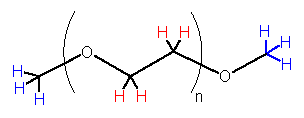
\includegraphics[width=0.35\textwidth]{\figpath/Model1-PEG}}
		
		\vspace{-8pt}
		The protons inside the repeat unit (red) are \emph{methylene} protons, while the protons on the end groups (blue) are \emph{methyl} protons.
		
		\begin{enumerate}
			\item How many methylene protons does this polymer have?  Give your answer in terms of the number of repeat units, $n$.
			
				\begin{solution}[0.5in]
					4n
				\end{solution}
			
			\item How many methyl protons does this polymer have?
			
				\begin{solution}[0.5in]
					6
				\end{solution}
			
			\item The intensity measured in NMR, $I$, is proportional to the number of protons of each type.  That is, 
				\begin{align*}
					I_{methylene} &= A \times (\text{\# of methylene protons})\\
					I_{methyl} &= A \times (\text{\# of methyl protons})
				\end{align*}
				so
				\begin{equation*}
					\frac{I_{methylene}}{I_{methyl}} = \frac{\text{\# of methylene protons}}{\text{\# of methyl protons}}
				\end{equation*}
				Substitute your answers to parts (a) and (b) into this expression, and then solve for $n$ in terms of the ratio $\frac{I_{methylene}}{I_{methyl}}$.
			
				\begin{solution}[1.25in]
					\begin{align*}
						\frac{I_{methylene}}{I_{methyl}} = \frac{4n}{6} && \text{so} && n = \frac{6}{4}\frac{I_{methylene}}{I_{methyl}}
					\end{align*}
				\end{solution}
				
			\item Suppose an NMR measurement on poly(ethylene glycol) dimethyl ether yields the following intensities for the methylene and methyl protons, respectively:
				\begin{align*}
					I_{methylene}=90 && \text{and} &&
					I_{methyl}=3
				\end{align*}
				Based on this information, and the approach you explored above, what must the degree of polymerization and the molecular weight of the polymer be?
				
				\emph{For ethylene glycol, the (\ce{CH2CH2O}) repeat unit has mass $M_0=44\text{ g/mol}$.}
				
				\begin{solution}[1.5in]
					Using the calculation from the previous part, we find that $n = (6/4)(90/3) = 45$.
					
					Multiplying by 44 g/mol, we obtain $M_n = (44\text{ g/mol})(45) = 2.0\text{ kg/mol}$.
				\end{solution}
				
		\end{enumerate}
		
		\question Briefly summarize how you could use NMR to determine the molecular weight of a polymer sample, if you are given its chemical structure.
		
			\begin{solution}[2in]
			\end{solution}
		
		\question It is difficult to determine the intensities of peaks in NMR spectra accurately if they are less than about 1\% of the intensity of the largest peaks.  Do you expect this to place any limits on the range of molecular weights that can be quantified by NMR?  Briefly explain your reasoning in 2-3 complete sentences.
		
			\begin{solution}[2in]
				Yes, this will limit the range of molecular weights that can be quantified by NMR.  If it is difficult to detect intensities of less than 1\%, then practically speaking, it will be difficult to quantify the number of end group protons when there are more than about 100 repeat units (though this limit may be larger or smaller depending on the number of protons contributing to each NMR peak).  For most polymers, this will limit the accessible range of molecular weights to around 10~kg/mol.
			\end{solution}
	
\end{ctqs}



\begin{model}[MALDI Mass Spectrometry]
	\label{\labelbase:mdl:MALDI}

	As you learned in Model \ref{\labelbase:mdl:endgrpanalysis}, end group analysis yields the number-average molecular weight of the polymer.  Often, however, it is more useful to measure the \emph{full distribution} of molecular weights.
	
	One technique that can be used to measure the full distribution of molecular weights is \emph{matrix-assisted laser desorption-ionization (MALDI) mass spectrometry}.  In this approach, depicted below, the polymer sample is deposited on a metal target.  A laser is then used to desorb individual polymer chains from the surface and ionize them (give them a charge):   
	
	\vspace{12pt}
	\centerline{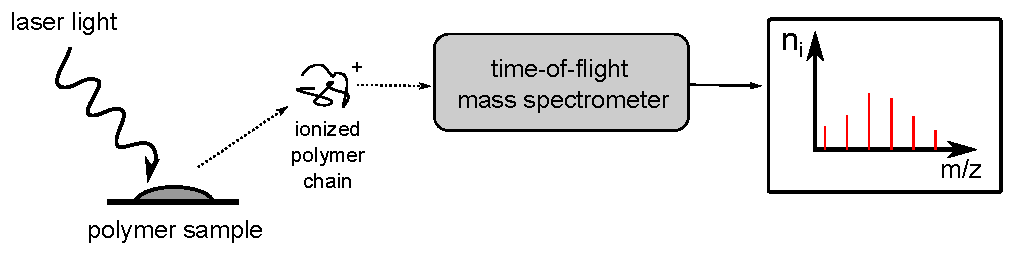
\includegraphics[width=0.7\textwidth]{\figpath/Model2-MALDIschematic}}
	
	The ionized polymer chains are then passed into a \emph{mass spectrometer}, which separates them by their mass-to-charge ratios, $m/z$.  The resulting mass spectrum contains a peak at each measured mass-to-charge ratio, with the intensity of each peak proportional to the number of chains with that $m/z$. 

\end{model}

\begin{ctqs}

	\question Suppose a polymer sample contains the following four polymer chains: \label{\labelbase:ctq:PS-MALDI}
	
			\centerline{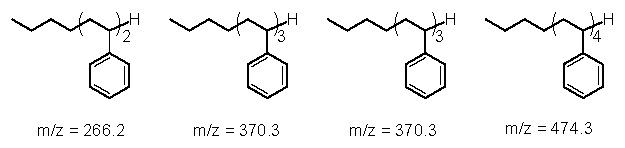
\includegraphics[width=0.85\textwidth]{\figpath/Model2-PSmz}}
	
		Plot the mass spectrum that you would measure for this sample (i.e. number of chains as a function of mass-to-charge ratio) on the following axes.  Make sure to clearly indicate that the number of chains is zero for any m/z values not present in the sample.
		
			\vspace{12pt}
			\centerline{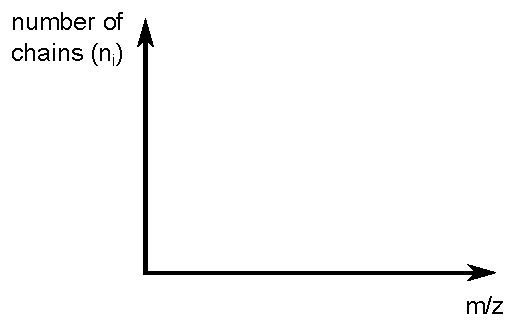
\includegraphics[width=0.4\textwidth]{\figpath/Model2-axes-v1}}
			
	\clearpage
	\question The mass spectrum you plotted in the previous question should have sharp peaks at three different $m/z$ ratios.
	
		\begin{enumerate}
			\item Calculate the \emph{difference} in the $m/z$ values for each adjacent pair of peaks.
			
				\begin{solution}[0.75in]
					Each pair of peaks is separated by 104.0 or 104.1 mass units
				\end{solution}
			
			\item How is the gap between peaks that you calculated in part (a) related to the molecular weight of the repeat unit in this polymer?
			
				\emph{Hint: remember that for styrene, $M_0 = 104\text{ g/mol}$!}
			
				\begin{solution}[0.75in]
					The gap is equal to the repeat unit molecular weight.
				\end{solution}
			
		\end{enumerate}
		
	\question Assuming each polymer chain has only a single charge, $m/z$ for a polymer chain is equal to its mass $M_i$.
	
		\begin{enumerate}
			\item Re-draw the mass spectrum you sketched in CTQ \ref{\labelbase:ctq:PS-MALDI} on the following axes:
		
			\vspace{12pt}
			\centerline{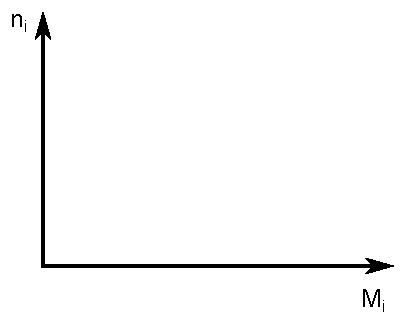
\includegraphics[width=0.4\textwidth]{\figpath/Model2-axes-v2}}
			
			\item Recall that the number-average and weight-average molecular weights of a polymer sample can be expressed as
		\begin{align*}
			M_n = \frac{\sum_i n_i M_i}{\sum_i n_i} && M_w = \frac{\sum_i n_i M_i^2}{\sum_i n_i M_i}
		\end{align*}
		where $n_i$ is the number of chains with length $i$ and $M_i$ is the mass of each chain that has length $i$.
		
				Using these equations, and the mass spectrum you sketched in the previous part, calculate $M_n$ and $M_w$ for this polymer sample in the space on the next page.
		\end{enumerate}
		
		%(calculation space, cont'd $\rightarrow$)
		\begin{solution}[3.5in]
			\begin{align*}
				M_n &= \frac{1\cdot 266.2 + 2\cdot 370.3 + 1\cdot 474.3}{1 + 2 + 1} = 370.3\\
				M_w &= \frac{1\cdot 266.2^2 + 2\cdot 370.3^2 + 1\cdot 474.3^2}{1\cdot 266.2 + 2\cdot 370.3 + 1\cdot 474.3} = 384.9
			\end{align*}
		\end{solution}
		
	\question Briefly summarize, in 2-3 complete sentences, how you could use a MALDI spectrum to obtain information about each of the following:
	
		\begin{enumerate}
			\item ... the molecular weight and dispersity of a polymer sample?
		\begin{solution}[2in]
		\end{solution}
				
			\item ... the repeat unit of a polymer if you \emph{did not} already know its structure?
		\begin{solution}[2in]
		\end{solution}
		
		\end{enumerate}
		
	%\question It is typically much easier to ionize smaller polymer molecules than it is to ionize larger polymer molecules.
		
\end{ctqs}



\begin{model}[Size-Exclusion Chromatography]
\label{\labelbase:mdl:SEC}
	
	Another popular approach to measuring the full distribution of molecular weights is \emph{size-exclusion chromatography} (SEC).
	In an SEC experiment, a solution of the polymer of interest is passed through a column containing a gel with many small pores:
	
	\vspace{12pt}
	\centerline{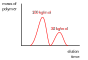
\includegraphics[width=0.6\textwidth]{\figpath/Model3-SEC}}
	
	As depicted in this image, small/compact polymer chains are able to get into many of the pores in the gel, while large polymer chains may be excluded from some or all of the pores on the basis of their size.

\end{model}

\begin{ctqs}

	\question Based on the image shown in Model \ref{\labelbase:mdl:SEC}, which type polymer (smaller or larger) travels a longer path as it passes through the gel?
	
		\begin{solution}[0.5in]
			smaller
		\end{solution}
	
	\question Based on your answer to the previous question, which type of polymer (smaller or larger) do you expect to take longer to elute (make it to the end of the column)?
	
		\begin{solution}[0.5in]
			smaller
		\end{solution}
	
\end{ctqs}

\begin{infobox}
	One of the most common types of detectors for an SEC instrument is a \emph{differential refractometer}.  The signal measured by this detector is proportional to the \emph{total mass} of polymer coming off the column at each elution time.
\end{infobox}

\clearpage
\begin{ctqs}
	
	\question Suppose a polymer sample contains 1~g of 30~kg/mol polystyrene, and 2~g of 100~kg/mol polystyrene.  On the following axes, sketch the shape of the SEC trace you would expect to measure for this sample.  Make sure to clearly label each peak with the molecular weight of the polymer to which it corresponds.
	
		\begin{solution}[2in]
		\studentdisplay{
			\vspace{12pt}
			\centerline{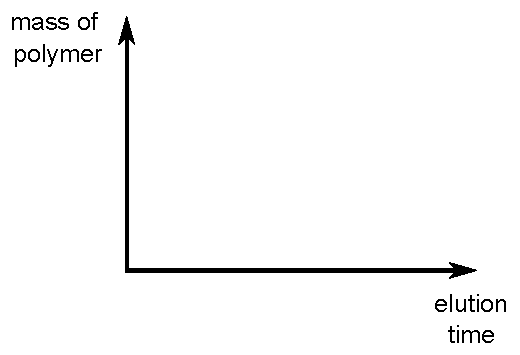
\includegraphics[width=0.5\textwidth]{\figpath/Model3-SECaxes}}
		}\instructordisplay{
			\vspace{12pt}
			\centerline{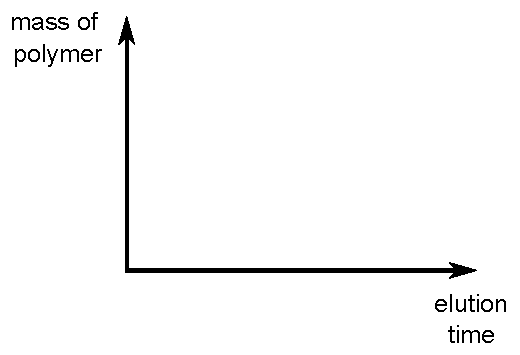
\includegraphics[width=0.5\textwidth]{\figpath/Model3-SECaxes}}
		}
		\end{solution}
	
	\question Propose methods that you could use to...
	
		\begin{enumerate}
			\item ... determine a calibration that would allow you to convert the x axis of this plot from elution time to molecular weight:
	
				\begin{solution}[1in]
					You could inject a series of polymers with known molecular weights and plot the resulting elution time vs. molecular weight.  You could then fit this data to an appropriate function(*) to make a calibration curve.
					
					(*) Retention time (and retention volume) have a logarithmic dependence on molecular weight, so the correct functional form is typically $V_R = A - B \log M$.
					
				\end{solution}
			
			\item ... convert the y axis from total mass to number of chains:
	
				\begin{solution}[1in]
					You would divide the total mass of polymer at each elution time by the molecular weight \emph{corresponding to that elution time}.
				\end{solution}
			
			\item ... calculate $M_n$ and $M_w$ from an SEC trace:
	
				\begin{solution}[1.5in]
					Once the axes have been converted to $M_i$ and $n_i$ as described above, you could just use the expressions for $M_n$ and $M_w$ from earlier in the activity, where the sum would be over \emph{each data point} in the SEC trace.
				\end{solution}
		
		\end{enumerate}
	
	\clearpage
	\question The size of a polymer chain in solution depends not only on the mass of the chain, but also on how favorable the polymer/solvent interaction is.  In a ``good'' solvent, a polymer chain will swell/expand to a larger size, while in a ``poor'' solvent, a polymer chain will deswell/contract to a smaller size.
	
		Based on this information, do you expect the same calibration to be valid for polymers with different chemical structures?  Briefly explain your group's reasoning in 2-3 complete sentences.		
	
			\begin{solution}[1.5in]
				No.  Suppose the calibration is calculated using a polymer for which the SEC solvent is a good solvent.  If we then analyze a different polymer, for which the SEC solvent is a poor solvent, the chains will be more compact and will take longer to elute from the column than chains of the same molecular weight did when we measured the calibration curve.  As a result, our calibration would determine the molecular weight of the polymer to be much lower than it actually is.
				
				While there are ways around this problem (e.g. universal calibration, using a light scattering detector in addition to a differential refractometer, etc.), the calibration should ideally be measured using known standards for each polymer/solvent pair.
			\end{solution}
	
	% \question Would also like a qualitative question about how peak shape relates to dispersity, but am not sure it fits in easily here - save for exercises?
	
	% \question Would also like a qualitative question about the relative resolution of SEC vs. MALDI, and fact that SEC can get to higher molecular weights...
	
\end{ctqs}


\begin{exercises}

	% \exercise The UV-VIs problem I removed from the earlier version of the activity
	
	\exercise Another technique used to quantify the molecular weights of polymers is light scattering.  In a light scattering experiment, the intensity of the signal from each polymer chain is proportional to the molecular weight of the chain.
	
		Based on this information, do you expect the molecular weight obtained from a light scattering measurement to be $M_n$ or $M_w$?  Explain your reasoning in 2-3 complete sentences.
		
	% \exercise A question getting students to think about why the TOF part of MALDI-TOF works to separate polymers by mass
	
	% \exercise A question getting students to think about how/why the fact that it is easier to ionize smaller chains affects MALDI interpretation
	
	\exercise Ionizing hydrophobic polymers such as polystyrene can be difficult.  To solve this problem, the polymers are often complexed with an ion such as silver.
	
		How would you expect the presence of a silver ion to change the mass spectrum you sketched in CTQ \ref{\labelbase:ctq:PS-MALDI}?  Briefly explain your reasoning in 2-3 complete sentences.
		
	% \exercise The question where we convert the Mn and Mw equations to concentrations for SEC analysis
	
\end{exercises}


	
\end{activity}